根据书本公式(5-9):

$$
\begin{cases}
\dot{v} = ((k_1+k_2)\frac{v}{n}+\frac{1}{u}(ak_1-bk_2)\omega_r -k_1\delta)/m-u\omega_r \\
\dot{\omega_r}=((ak_1-bk_2)\frac{v}{u}+\frac{1}{u}(a^2k_1+b^2k_2)\omega_r-ak_1\delta)/I_z
\end{cases}
$$    

使用simulink中的Matlab function模块,编写出$\dot{v},\dot{\omega_r}$关于$v,\omega_r,\delta,u$的方程。

\begin{figure}[h]
    \centering
    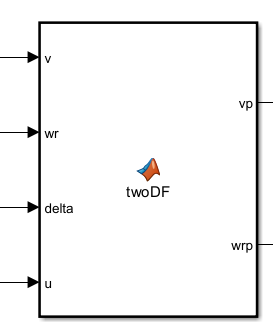
\includegraphics[width=2.5cm]{figure/fcn.png}
    \caption{Matlab function 模块}
    \label{matlabfcn}
\end{figure}

其中$v$和$\omega_r$分别由$\dot{v}$和$\dot{\omega_r}$积分得到。在第五章的特定条件下,汽车$x$轴的前进速度$u$视为不变,$\delta$手动设置以研究不同操作下车辆模型的响应。最终线性二自由度汽车simulink模型如下图所示

\begin{figure}[h]
    \centering
    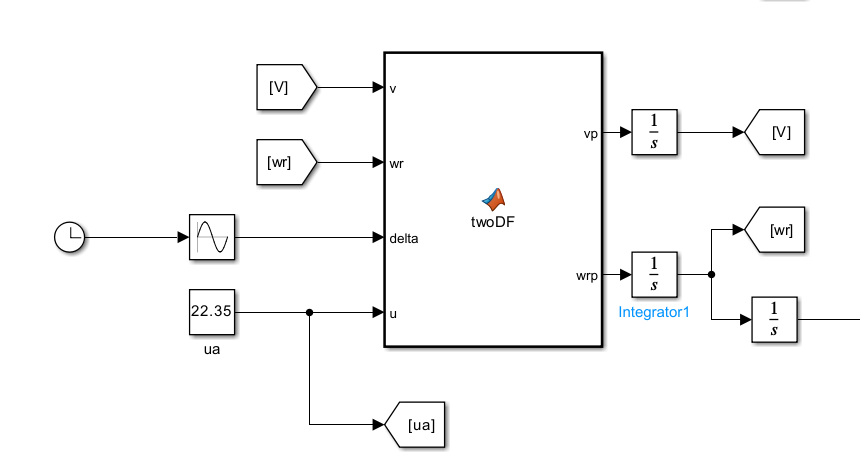
\includegraphics[width=5.5cm]{figure/2DF.png}
    \caption{线性二自由度汽车模型}
    \label{2DF}
\end{figure}

